\documentclass[aspectratio=169]{beamer}
\usepackage[utf8]{inputenc}
\usepackage{amsmath}
%\usepackage[ngerman]{babel}
\usepackage{xcolor}
\usepackage{listings}
%\usepackage[automark]{scrpage2}
\usepackage[]{graphicx, import} 
\usepackage{subfigure}
\usepackage{wrapfig}
\usepackage[scaled]{helvet}
\renewcommand*\familydefault{\sfdefault}
%\usepackage{enumitem}
\usepackage[comma]{natbib}
\usepackage{url}
\usepackage{import}
\usepackage{gensymb}
\bibliographystyle{dcu}
%\citationstyle{dcu}
%\setbeamertemplate{footline}[page number]
\usetheme{FHNW}
\usecolortheme{seagull}
\usepackage{multimedia}

\usepackage{hyperref}




\begin{document}
% infos for pdf document settings
\pdfinfo{
/Author (Stefan Blaser, FHNW - IVGI)
/Title (Development of an Acquisition Software 
	for our Image-Based Indoor Mobile Mapping System 
	based on the Robot Operating System (ROS))
/Subject (GeoPython 2017)
/Keywords (ROS, Mobile Mapping, Indoor, Python)}

% infos for title page
\title{\textbf{Development of an Acquisition Software
	for our Image-Based Indoor Mobile Mapping System 
	based on the Robot Operating System (ROS)}}
\subtitle{GeoPython 2017}
\author{Stefan Blaser}
\institute{Institute of Geomatics Engineering}
\date{\today}

% title page
\begin{frame}
 \titlepage
\end{frame}

\section{Introduction}

% Frame 2: Mobile Mapping
  \begin{frame}
   \frametitle{Introduction}
   \begin{columns}[onlytextwidth]

    \begin{column}{0.5\textwidth}
    Mobile Mapping
      \begin{itemize}
       \item Image-based Mobile Mapping \newline(since 2011 @ FHNW)
       \item Spin-off company iNovitas
       \item ``Google Street View''-like service
       \item Measurement functionality
       \item Measurement accuracy:
       \begin{itemize}
        \item relative: ca. $1\, cm$
        \item absolute: ca. $3-5\, cm$ \newline(GNSS accuracy)
       \end{itemize}
       \citep{Burkhard2012}
      \end{itemize}
    \end{column}
    \begin{column}{0.5\textwidth}
    
     \begin{figure}[h]
       \centering
       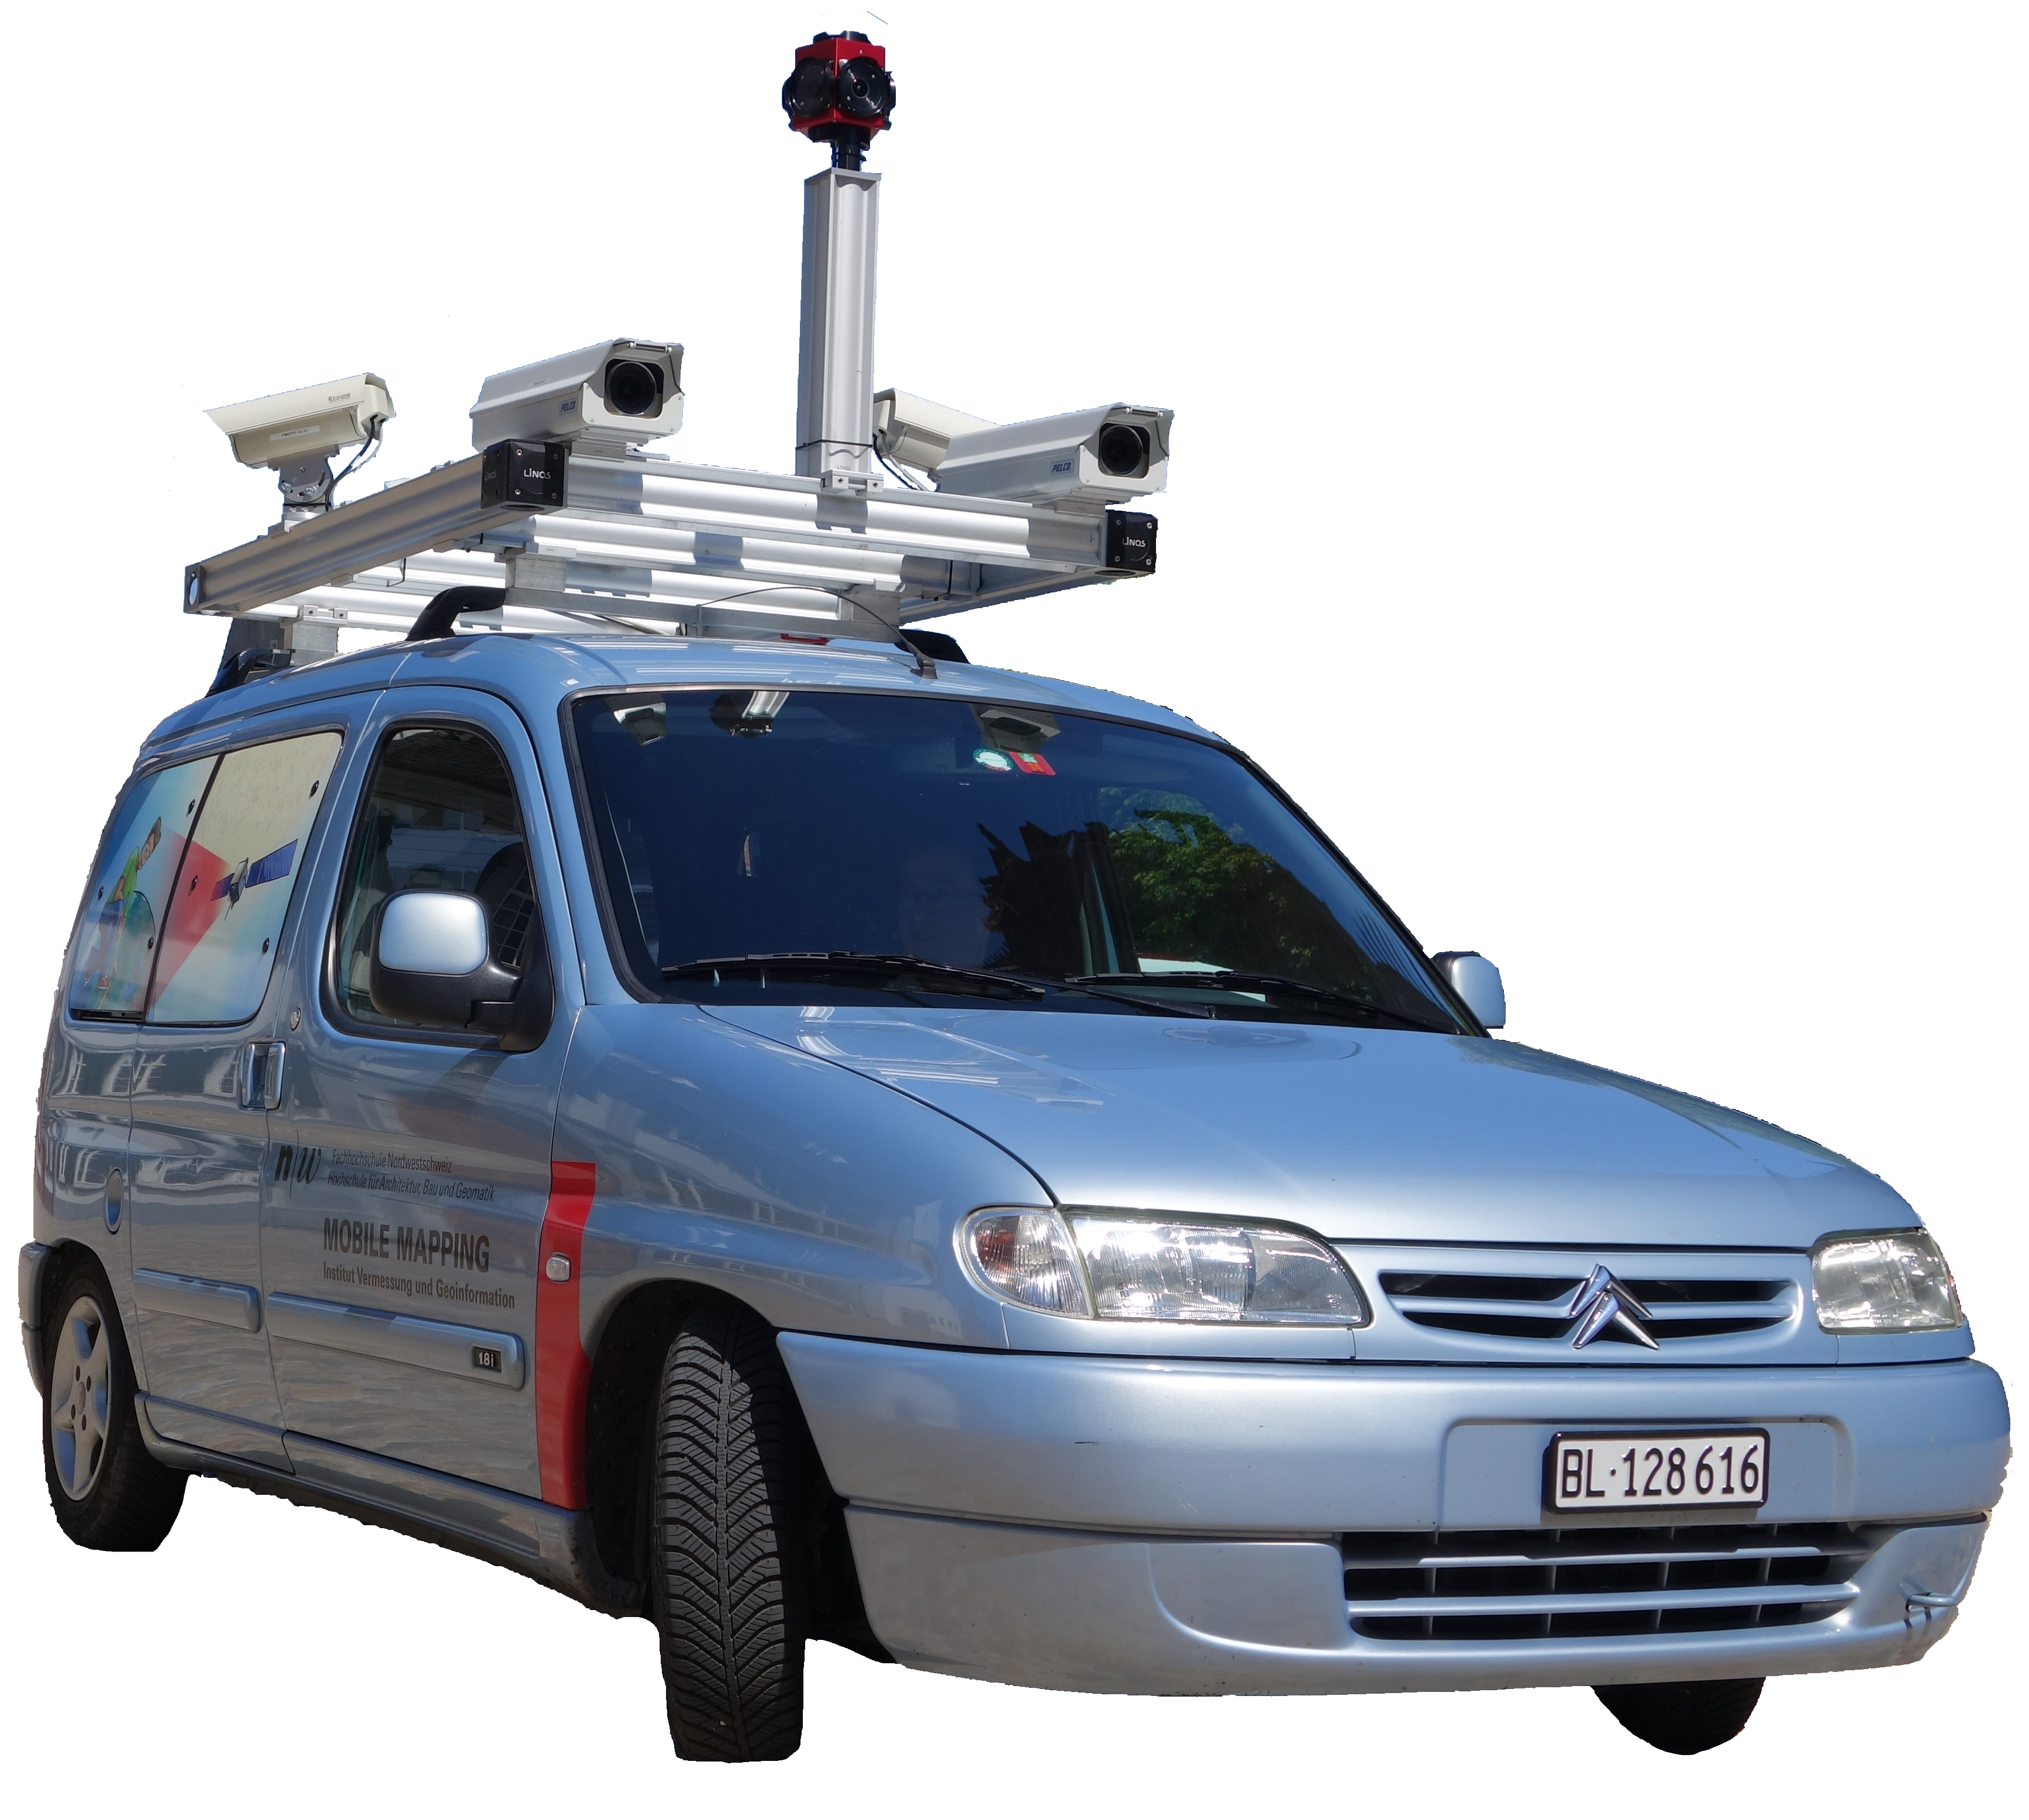
\includegraphics[width=5.5cm]{./Abbildungen/mms.png}
       \caption{Mobile Mapping vehicle of FHNW}
       \label{abb:mms}
     \end{figure}
     
    \end{column}
    
   \end{columns}
  \end{frame}

% Frame 3: CTI-Project BIMAGE
  \begin{frame}
   \frametitle{Introduction}
   \begin{columns}[onlytextwidth]

    \begin{column}{0.5\textwidth}
    CTI project ``BIMAGE''
      \begin{itemize}
       \item Main Goal: 
       \begin{itemize}\item Transfer outdoor technology into interior spaces\end{itemize}
       \pause
       \item Deliverables:
       \begin{itemize}
        \item \textbf{Indoor Mobile Mapping System} (IMMS) (absence of GNSS) \pause
        \item Software to follow changes using mobile devices \pause
        \item New navigation concepts for cloud application \pause
        \item Sophisticated photogrammetric image post-processing approaches 
       \end{itemize}
      \end{itemize}
    \end{column}
    \begin{column}{0.5\textwidth}
    \begin{center}
    \includegraphics[width=0.9\textwidth]{./Abbildungen/FHNW_HABG_10mm.jpg} \\
    % FHNW_HABG_10mm.jpg: 0x0 pixel, 300dpi, 0.00x0.00 cm, bb=
    \includegraphics[width=0.2\textwidth]{./Abbildungen/iNovitas_Logo.png} \\
    % iNovitas_Logo.png: 0x0 pixel, 300dpi, 0.00x0.00 cm, bb=
    \includegraphics[width=0.7\textwidth]{./Abbildungen/F&E_Absender_Dritte_Un_D_1200.png}
% F&E_Absender_Dritte_Un_D_1200.png: 0x0 pixel, 300dpi, 0.00x0.00 cm, bb=
    \end{center}
    
    \end{column}
    
   \end{columns}
  \end{frame}


\section{Software Requirements}

  \begin{frame}
   \frametitle{Indoor mobile mapping system prototype}
   \begin{columns}[onlytextwidth]
    \begin{column}{0.5\textwidth}
      \def\svgwidth{5.5cm}
      \input{./Abbildungen/imms_explanation.pdf_tex}
    \end{column}
    \begin{column}{0.5\textwidth}
      \begin{itemize}
        \item multi sensor system
	\item weight: $30\,kg$ ($66.1\, lbs$)
	\item research prototype
	\item hardware components might change during project time
       \pause
       \item acquisition software requirements:
       \begin{itemize}
       \item Modular software architecture
       \item Free open source software (FOSS)
       \item Existing modules for hardware support
       \end{itemize}
      \end{itemize}
    \end{column}

   \end{columns}
  \end{frame}

\section{Robot Operating System (ROS)}

  \begin{frame}
   \frametitle{Robot Operating System (ROS)}
   \begin{columns}[onlytextwidth]
    \begin{column}{0.5\textwidth}
    
      \begin{itemize}
       \item Software framework for robots 
       \item Free and Open-Source 
       \item Graph-based communication layer 
       \item Collection of tools and libraries 
       \item Multi-lingual 
       \begin{itemize}
	\item C++
	\item \textbf{Python} 
       \end{itemize}
       \cite{Quigley2009}
       \item \url{www.ros.org}
      \end{itemize}
    
    \end{column}
    \begin{column}{0.5\textwidth}

    \includegraphics[width=1.5\textwidth]{./Abbildungen/ros_screenshot.png}
    % ros_screenshot.png: 0x0 pixel, 300dpi, 0.00x0.00 cm, bb=
    
    \end{column}
   \end{columns}
  \end{frame}

  \begin{frame}
   \frametitle{Graph-based communication layer}
   \begin{columns}[onlytextwidth]
    \begin{column}{0.5\textwidth}
    
      \begin{description}
       \item [\textbf{Node}] software module, process
       \item [\textbf{Messages}] data in a predefined structure
       \item [\textbf{Topic}] where messages go through
       \item [\textbf{Service}] allows synchronous communication (request / response)
      \end{description}
       
    \end{column}
    \begin{column}{0.5\textwidth}

      \begin{figure}[h]
	\centering
	\includegraphics[width=\textwidth]{./Abbildungen/ROS-Graph-basic.png}
	% ROS-Graph-basic.png: 0x0 pixel, 300dpi, 0.00x0.00 cm, bb=
	\caption{ROS communication principle}
	\label{abb:graph}
      \end{figure}
    \end{column}
   \end{columns}
  \end{frame}

\section{Implemented Acquistion Software}

  \begin{frame}
   \frametitle{Acquisition software design}
    
    \begin{figure}[h]
      \centering
      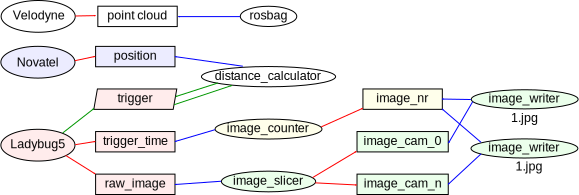
\includegraphics[width=13.5cm]{./Abbildungen/ROSImageCapturing.png}
      % ROSImageCapturing.png: 0x0 pixel, 300dpi, 0.00x0.00 cm, bb=
      %\caption{Graph-based software design of the image acquisition part}
      \label{abb:ROSImageCapturing}
    \end{figure}

  \end{frame}
  
  \begin{frame}
   \frametitle{Acquisition software design}
    
    \begin{figure}[h]
      \centering
      \includegraphics[width=13.5cm]{./Abbildungen/ROSImageCapturingFrame.png}
      % ROSImageCapturing.png: 0x0 pixel, 300dpi, 0.00x0.00 cm, bb=
      %\caption{Graph-based software design of the image acquisition part}
      \label{abb:ROSImageCapturingFrame}
    \end{figure}

  \end{frame}

% Python listings image event counter
\defverbatim[colored]\lstOne{
  \begin{lstlisting}[language=python, basicstyle=\ttfamily, keywordstyle=\color{blue}]
#!/usr/bin/env python
import rospy
from std_msgs.msg import *

class ImageEventCounter():
    [...]

def main():
    [...]

if __name__ == '__main__':
    main()
  \end{lstlisting}
}
\defverbatim[colored]\lstTwo{
  \begin{lstlisting}[language=python, basicstyle=\ttfamily, keywordstyle=\color{blue}]
def main():
    rospy.init_node("ImageEventCounter", 
                    anonymous=True)
    image_event_counter_node = ImageEventCounter()
    try:
        rospy.spin()
    except KeyboardInterrupt:
        pass
  \end{lstlisting}
}
\defverbatim[colored]\lstThree{
  \begin{lstlisting}[language=python, basicstyle=\ttfamily, keywordstyle=\color{blue}]
class ImageEventCounter():
    def __init__(self):
        # read out parameter
        self.counter = \
            rospy.get_param('counter_start', 0)
        subscriber_tn = \
            rospy.get_param('subscriber_name', 
                            '/trigger_time')
        publisher_tn = \
            rospy.get_param('publisher_name', 
                            '/image_nr')
	[...]
  \end{lstlisting}
}
\defverbatim[colored]\lstFour{
  \begin{lstlisting}[language=python, basicstyle=\ttfamily, keywordstyle=\color{blue}]
class ImageEventCounter():
    def __init__(self):
	[...]
	self.trigger_time_sub = \
	    rospy.Subscriber(subscriber_tn,
                             Time,
                             self.subscriber_callback)
        self.trigger_count_pub = \
	    rospy.Publisher(publisher_tn,
                            UInt32,
                            queue_size=1)
    def subscriber_callback(self, time):
        [...]
  \end{lstlisting}
}
\defverbatim[colored]\lstFive{
  \begin{lstlisting}[language=python, basicstyle=\ttfamily, keywordstyle=\color{blue}]
class ImageEventCounter():
    def __init__(self):
	[...]
    def subscriber_callback(self, time):
        self.counter += 1
        self.trigger_count_pub(UInt32(\
                               self.counter))
  \end{lstlisting}
}

\begin{frame}
 \frametitle{ImageEventCounter -- node structure}
 \lstOne
\end{frame}

\begin{frame}
 \frametitle{ImageEventCounter -- main function}
 \lstTwo
\end{frame}

\begin{frame}
 \frametitle{ImageEventCounter -- read out parameter}
 \lstThree
\end{frame}

\begin{frame}
 \frametitle{ImageEventCounter -- publisher / subscriber}
 \lstFour
\end{frame}

\begin{frame}
 \frametitle{ImageEventCounter -- subscriber callback}
 \lstFive
\end{frame}

  \begin{frame}
   \frametitle{Controller node}
    
    \begin{figure}[h]
      \centering
      \includegraphics[width=13.5cm]{./Abbildungen/ROSImageCapturingGUI.png}
      % ROSImageCapturing.png: 0x0 pixel, 300dpi, 0.00x0.00 cm, bb=
      %\caption{Graph-based software design of the image acquisition part}
      %\label{abb:ROSImageCapturing}
    \end{figure}

  \end{frame}
  
  \begin{frame}
   \frametitle{Controller node}
    
    \begin{itemize}
     \item dynamic parameter changes
     \item change node settings
     \item launches and kills nodes
     \item GUI 
     \begin{itemize}
      \item developed with pyqt4
      \item put ROS node into pyqt4-loop
      \item \textit{rospy.spin()} becomes obivious
    \end{itemize}
    \end{itemize}

  \end{frame}
  
  \begin{frame}
   %\frametitle{Controller node -- GUI}
   \begin{center}
    \includegraphics[width=10cm]{./Abbildungen/GUI_1.png}
    % GUI_1.png: 0x0 pixel, 300dpi, 0.00x0.00 cm, bb=
   \end{center}
  \end{frame}
  
  \begin{frame}
   %\frametitle{Controller node -- GUI}
   \begin{center}
    \includegraphics[width=10cm]{./Abbildungen/GUI_2.png}
    % GUI_1.png: 0x0 pixel, 300dpi, 0.00x0.00 cm, bb=
   \end{center}
  \end{frame}

  \begin{frame}
   %\frametitle{Controller node -- GUI}
   \begin{center}
    \includegraphics[width=10cm]{./Abbildungen/GUI_3.png}
    % GUI_1.png: 0x0 pixel, 300dpi, 0.00x0.00 cm, bb=
   \end{center}
  \end{frame}
  
  \begin{frame}
   %\frametitle{Controller node -- GUI}
   \begin{center}
    \includegraphics[width=10cm]{./Abbildungen/GUI_4.png}
    % GUI_1.png: 0x0 pixel, 300dpi, 0.00x0.00 cm, bb=
   \end{center}
  \end{frame}
  
  \begin{frame}
   \frametitle{SLAM (post processing)}
   \begin{itemize}
    \item simultaneous localization and mapping (SLAM)
    \item different SLAM techniques (lidar-based, visual-based, ...)
    \item some SLAM algorithms are supporting loop closure
    \item possible subtitution of GNSS in indoor environment
    \pause
    \item Google cartographer
    \begin{itemize}
     \item lidar-based SLAM algorithm with IMU support
     \item Open source software since 05.10.2016
     \item ROS support
     \item both, 2D and 3D SLAM version \citep{Hess2016}
     \item loop closure
    \end{itemize}
   \end{itemize}
  \end{frame}
  
  \begin{frame}
   %\frametitle{SLAM (post processing)}
   \movie[showcontrols]{\includegraphics[width=1\textwidth]{./Abbildungen/Video.jpg}}{./Abbildungen/mymovie.mp4}
   %\movie[width=3cm,height=2cm,poster]{}{./Abbildungen/mymovie.mp4}
   %TODO insert right!!! video
  \end{frame}



\section{Conclusion and Outlook}

\begin{frame}
 \frametitle{Conclusion}
 \begin{itemize}
  \item IMMS acquisition software successfully implemented $\rightarrow$ based on ROS
  \item graph-based architecture $\rightarrow$ flexibility \pause
  \item numerous existing free open source ROS packages available
  \item from hardware node up to SLAM algorithm \pause
  \item wide ROS community $\rightarrow$ quasi-standard in robotics \pause
  \item learning curve
 \end{itemize}

\end{frame}

\begin{frame}
 \frametitle{Outlook}
 \begin{itemize}
  \item Indoor localization $\rightarrow$ Replacement of INS by SLAM
  \item real time SLAM
  \item weight loss about $10\,kg$
  \item use SLAM map as progress control
  \item replacement of ladybug5 camera by a stereo panorama camera
  \item several GUI optimizations
  \item ...
 \end{itemize}

\end{frame}

\begin{frame}
%\bibliography{20170510_GeoPython}
\frametitle{Literature}
\small\setbeamertemplate{bibliography item}[text]\bibliography{20170510_GeoPython}

\bibliographystyle{dcu}
%\renewcommand{\bibliography}
\end{frame}

\begin{frame}
 \frametitle{Thank you for your attention!}
 \begin{itemize}
  \item Questions?
 \end{itemize}
\end{frame}

\end{document}
